\chapter{Background :  The $\bar{B}\rightarrow X_s\gamma$ decay}
The inclusive radiative $\bar{B}\rightarrow X_s\gamma$ decay is an important new physics probe. Since this is a FCNC process, it does not occur at tree level in the SM. Therefore, it can be highly sensitive to new physics. In particular, these new physics sources can modify the Wilson coefficient $C_{7\gamma}$, and they may introduce new weak phases that can enhance the SM CP asymmetry.\par
The $b\rightarrow s\gamma$ is the underlying partonic decay of the inclusive $B\rightarrow X_s\gamma$ decay. This $b$ to $s$ transition is one of the most reliably calculable FCNC processes in SM \cite{Ritchie:2013xc}. The final states $X_s$ represent a final state that contains a $s$ quark\par
The current SM next to-next to leading (NNLO) prediction for the $\bar{B}\rightarrow X_s\gamma$ branching ration is $\mathcal{B}^{\rm{SM}}_{X_s\gamma}=(3.36\pm0.23)\times 10^{-4}$ \cite{Misiak:2015xwa, Czakon:2015exa}. The experimental world average is $\mathcal{B}^{\rm{exp}}_{X_s\gamma}= (3.32\pm0.15)\times 10^{-4}$ \cite{Amhis:2019ckw, Chen:2001fja, Aubert:2007my, Lees:2012wg, Lees:2012ym, Saito:2014das, Belle:2016ufb}. The experimental uncertainty on the branching ratio is expected to reduce from $\pm 4.5\%$ to around $\pm 2.6\%$ in future thanks to Belle II measurements \cite{Kou:2018nap}. With these new precision measurements, SM prediction can strongly constrain the BSM. Therefore, improving the precision of the theoretical prediction is important.\par

The uncertainty of the SM prediction  arise from several sources. These uncertainties were combined in quadrature to obtain the total uncertainty ($\pm 6.8\%$). The breakdown of these uncertainties is as follows:
The nonperturbative contribution to the uncertainty is $\pm 5\%$ \cite{Benzke:2010js}, parametric uncertainty is $\pm 2\%$, perturbative uncertainty is $\pm 3\%$, the uncertainty from interpolating the charm mass in two-loop is $\pm 3\%$ \cite{Czakon:2015exa}.\par

Since the nonperturbative uncertainty provides the largest contribution to the total uncertainty, we would like to explore the possibility of improving this estimate. The question that we are prompt to ask is ``how do we reduce this uncertainty?''. In the following work, we address the issue of reducing the nonperturbative contribution of the theoretical prediction.

\section{The inclusive decay rate}
The inclusive decay rate for the $\bar{B}\rightarrow X_s\gamma$ is obtained by using the optical theorem. This theorem relates the decay rate to the imaginary part of the forward scattering amplitude. The $\bar{B}\rightarrow X_s \gamma$ decay is can be written as
\begin{eqnarray}\label{eqn:Inclsv_dacay_rate_btoxgamm}
\Gamma\left(\bar{B} \rightarrow X_s\gamma\right)=\frac{1}{M_{B}} \operatorname{Im}\left\langle \bar{B}|\mathbf{T}| \bar{B}\right\rangle,
\end{eqnarray} 
where $\mathbf{T}$ is related to the effective Lagrangian. However, instead of effective Lagrangian we use the effective Hamiltonian ($\mathcal{H}_{\mathrm{eff}}$)
\begin{eqnarray}\label{eqn:Trans_matrix_btoxgam}
\mathbf{T}=i \int \mathrm{d}^{4} x T\left\{\mathcal{H}_{\mathrm{eff}}(x), \mathcal{H}_{\mathrm{eff}}(0)\right\}, 
\end{eqnarray}
where $\mathcal{H}_{\mathrm{eff}}$ is obtained after integrating out the $W$ boson \cite{Benzke:2010js}. The effective Hamiltonian is given by

\begin{equation}\label{eq:Weak Hamiltonian}
   {\cal H}_{\rm eff} = \frac{G_F}{\sqrt{2}} \sum_{q=u,c} \lambda_q\,
   \bigg( C_1\,Q_1^q + C_2\,Q_2^q + \sum_{i=3,...,6} C_i\,Q_i 
   + C_{7\gamma}\,Q_{7\gamma} + C_{8g}\,Q_{8g} \bigg) \,,
\end{equation}
where $\lambda_q=V_{qb} V_{qs}^*$, $C_{i}$ are the Wilson coefficients and $Q_i$ are the effective operators.
This Hamiltonian describes the underlying are weak interaction in the decay process.\par
The decay rate and the photon spectrum related to the restricted discontinuity of forward scattering matrix element \cite{Benzke:2010js}.
\begin{eqnarray}\label{eqn:discont_eval}
d \Gamma\left(\bar{B} \rightarrow X_{s} \gamma\right) \propto \operatorname{Disc}_{\mathrm{restr}}\left[i \int d^{4} x\left\langle\bar{B}\left|\mathcal{H}_{\mathrm{eff}}^{\dagger}(x) \mathcal{H}_{\mathrm{eff}}(0)\right| \bar{B}\right\rangle\right],
\end{eqnarray}
where the restricted discontinuity implies that the discontinuity is restricted by the requirement that the cut must be applied on photon and strange quark propagators. 
\subsection{Kinematics of the decay} 
In its rest frame, the $B$ meson is decaying into a hadronic jet, which carries a momentum $P_X$, and to a photon, which carries a momentum $q$. The momentum of the heavy hadron is $M_{B} v=P_{X}+q$, where $v$ is the four velocity of the $B$ meson. In the $B$ meson rest frame $v=(1,0,0,0)$. We can align $\vec{q}$ in the negative $z$ direction and define two light-like vectors $n^{\mu}=(1,0,0,1)$ and $\bar{n}^{\mu}=(1,0,0,-1)$. These $n$ and $\bar{n}$ vectors satisfy $\bar{n}+n=2v$, $\bar{n}\cdot n=2$ and $n\cdot v=\bar{n}\cdot n=1$ \cite{Paz:2009ut}. In general, any four vector can be decomposed as 
\begin{eqnarray}\label{eqn:4vec_decomp}
a^{\mu}=\bar{n} \cdot a \frac{n^{\mu}}{2}+n \cdot a \frac{\bar{n}^{\mu}}{2}+a_{\perp}^{\mu}.
\end{eqnarray}
For the choice of $v,n,\bar{n}$ the transverse component ($\perp$) is spanned by $(0,1,0,0)$ and $(0,0,1,0)$. These transverse indices can be contracted using
\begin{eqnarray}\label{eqn:Transverse_indices_contract}
g_{\perp}^{\mu \nu}=g^{\mu \nu}-\frac{n^{\mu} \bar{n}^{\nu}+n^{\nu} \bar{n}^{\mu}}{2}, \quad \epsilon_{\perp}^{\mu \nu}=\frac{1}{2} \epsilon^{\mu \nu \alpha \beta} \bar{n}_{\alpha} n_{\beta}
\end{eqnarray}
where we use the following convention for the levi-civita tensor $\epsilon_{0123}=1$.\par
The conservation of four momentum provides that there is only one independent kinematical variable in $\bar{B}\rightarrow X_s\gamma$ decay that is the photon energy $E_{\gamma}$.

\subsection{Factorization}
At the leading order the $\bar{B}\rightarrow X_s\gamma$ decay can be thought of as a decay of constituent $b$ quark decaying into an $s$ quark and a photon. This constituent quark decay is expressed by the electromagnetic dipole operator $Q_{7\gamma}$
\begin{eqnarray}
Q_{7\gamma} &= \frac{-e m_b}{8\pi^2}\bar s\sigma_{\mu\nu}(1+\gamma_5)F^{\mu\nu}b.
\end{eqnarray}
However, this is not the only way to produce a photon. For instance, a gluon or a quark pair that was produced at the weak vertex can be converted to a photon, and these processes are described by the operators $Q_{8 g}=\left(-g / 8 \pi^{2}\right) m_{b} \overline{s} \sigma_{\mu \nu} G^{\mu \nu}\left(1+\gamma_{5}\right) b$ and $Q_{1}^{c}=(\overline{c} b)_{V-A}(\overline{s} c)_{V-A}$ respectively. The effective Hamiltonian for $\bar{B}\rightarrow X_{s}\gamma$ needs to account for all of these operators to accutrately describe the decay process.\par
The major contribution to the effective Hamiltonian arises from the operators $Q_{1}^{q}, Q_{7\gamma}$ and $Q_{8g}$ \cite{Benzke:2010js}. This is because the Wilson coefficients of these operators are relatively larger than the rest.\par
At the leading order the only the operator pair $Q_{7\gamma}-Q_{7\gamma}$ contributes to the decay rate. The contributions from operators such as $Q_1^q$ and $Q_{8g}$ give higher order contributions, and they either ``cost" a factor of $\alpha_s$ or $1/m_{b}$ in the decay rate calculation.\par
The shape of the $\bar{B}\rightarrow X_s\gamma$ photon spectrum probes the nonperturbative hadronic physics in the decay. At the leading order this photon spectrum is related to a universal shape function that parametrizes the $b$ quark momentum in the $B$ meson bound state. This shape function also parameterizes the leading order bound state effects of semileptonic decay $\bar{B}\rightarrow X_u l \nu$. However, the contributions of operators other than $Q_{7\gamma}-Q_{7\gamma}$ to  $\bar{B}\rightarrow X_s\gamma$ make the analysis of the photon spectrum more involved than the semileptonic $\bar{B}\rightarrow X_u l \nu$ decays. This is manifested in their corresponding factorization theroms. For instance, the factorization theorem for the $\bar{B}\rightarrow X_u l \nu$ decay in the end point region can be schematically expressed as follows \cite{Korchemsky:1994jb, Bauer:2001yt, Bosch:2004th}:
\begin{eqnarray}\label{eqn:inclsv_semiLp_fact}
d \Gamma\left(\bar{B} \rightarrow X_{u} l \bar{\nu}\right)=\sum_{n=0}^{\infty} \frac{1}{m_{b}^{n}} \sum_{i} H_{i}^{(n)} J_{i}^{(n)} \otimes S_{i}^{(n)},
\end{eqnarray}
where the hard functions $H_i^{(n)}$ paramterize the physics at the scale of $m_b$, the jet functions $J_i^{(n)}$ provides the physics of hadronic final state $X_u$, which has the invariant mass $M_X\sim \sqrt{m_b\Lambda_{\rm{QCD}}}$, and the soft function $S_i^{(n)}$ describes the hadronic physics at the scale $\Lambda_{\rm{QCD}}$. These soft functions are defined as forward scattering non-local HQET matrix elements. The symbol $\otimes$ represents convolusion \cite{Benzke:2010js}.\par
The higher order processes that were discussed above are known as \textit{resolved photon contributions} \cite{Benzke:2010js}. These processes describe the photon coupling to light partons instead of directly connecting to the effective weak vertex. The presence of the resolved photon contributions complicates the decay rate calculation compared to the processes that contain only the direct photon coupling processes. By considering all these effects the factorization theorem for the $\bar{B}\rightarrow X_s\gamma$ decay can be schematically represented as \cite{Benzke:2010js}:
\begin{align}\label{eqn:btoxgam_fact}
d \Gamma\left(\bar{B} \rightarrow X_{s} \gamma\right) &=\sum_{n=0}^{\infty} \frac{1}{m_{b}^{n}} \sum_{i} H_{i}^{(n)} J_{i}^{(n)} \otimes S_{i}^{(n)}\nonumber\\
&+\sum_{n=1}^{\infty} \frac{1}{m_{b}^{n}}\left[\sum_{i} H_{i}^{(n)} J_{i}^{(n)} \otimes S_{i}^{(n)} \otimes \bar{J}_{i}^{(n)}+\sum_{i} H_{i}^{(n)} J_{i}^{(n)} \otimes S_{i}^{(n)} \otimes \bar{J}_{i}^{(n)} \otimes \bar{J}_{i}^{(n)}\right].\nonumber\\
\end{align}
Note that equation (\ref{eqn:btoxgam_fact}) contains both direct contributions, which are similar to the contributions present in equation (\ref{eqn:inclsv_semiLp_fact}), and resolved photon contributions. The resolved photon contributions probe the hadronic substructure of the photon at the scale $\sqrt{2 E_{\gamma} \Lambda_{\mathrm{QCD}}}$. The effect of these new sub-processes requires new jet functions $\bar{J}_i^{(n)}$. In equation (\ref{eqn:btoxgam_fact}), we find two types of resolved photon contributions. The term $\sum_{i} H_{i}^{(n)} J_{i}^{(n)} \otimes S_{i}^{(n)} \otimes \bar{J}_{i}^{(n)}$ refers to single resolved photon contribution. Whereas, the term $\sum_{i} H_{i}^{(n)} J_{i}^{(n)} \otimes S_{i}^{(n)} \otimes \bar{J}_{i}^{(n)} \otimes \bar{J}_{i}^{(n)}$ refers to double resolved photon contributions. The graphical illustration of $\bar{B}\rightarrow X_s\gamma$ factorization is provided in the figure \ref{fig:factorization}
\begin{figure}[H]
\centering
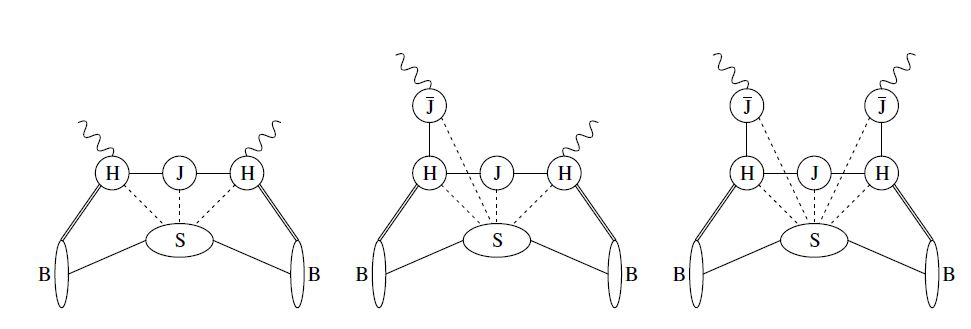
\includegraphics[width=15cm]{Factorization.JPG}
\caption{\label{fig:factorization} Graphical illustration of the factorization for $\bar{B}\rightarrow X_s\gamma$ decay \cite{Benzke:2010js}
}
\end{figure}
Note that this notation is symbolic. Because of this different quantities in different terms can be represented by the same symbol. 

\subsection{Review of the known results}
The factorization formula for the CP-averaged $\bar{B}\rightarrow X_s\gamma$ photon spectrum at the end point region is  
\begin{equation}\label{eqn:chap3_photon_spectrum}
\begin{aligned}
   \frac{d\Gamma}{dE_\gamma} 
   &= \frac{G_F^2\alpha|V_{tb} V_{ts}^*|^2}{2\pi^4}\,
    \overline{m}_b^2(\mu)\,E_\gamma^3\,\Bigg[\,
    |H_\gamma(\mu)|^2 \int_{-p_+}^{\bar\Lambda}\!d\omega\,m_b\,
    J\big( m_b(\omega+p_+),\mu \big)\,S(\omega,\mu) \\
   &\hspace{4.9cm}\mbox{}+ \frac{1}{m_b}\,\sum_{i\le j}\,
    \mbox{Re}\big[C_i^*(\mu)\,C_j(\mu)\big]\,F_{ij}(E_\gamma,\mu)
    + \dots \Bigg] \,,
\end{aligned}
\end{equation}
where $p_{+} \equiv m_{b}-2 E_{\gamma}=\mathcal{O}\left(\Lambda_{\mathrm{QCD}}\right)$, $\bar{\Lambda}$ is defined as $\bar{\Lambda}=M_{B}-m_{b}$ and the ellipses denotes the order $1/m_{b}^2$ terms. The $b$ quark mass is defined in the $\overline{\rm{MS}}$ scheme (see appendix \ref{app:Wilson} ). \par
The first line in the equation represents the leading power contribution, and an extensive discussion regarding this contribution can be found in \cite{Paz:2009ut, Paz:2006me}. The hard function $H_{\gamma}(\mu)$ is the matching coefficient, and it is $H_{\gamma}(\mu)=C_{7\gamma}(\mu)+\mathcal{O(\alpha)}$. In particular, this was obtained by matching the leading current operator to the soft collinear effective field theory (SCET). Also, this current receives contributions from all the operators in the effective Hamiltonian. The dominant contribution is received from $Q_{7\gamma}$, and this is known to $\mathcal{O}(\alpha_s^2)$ \cite{Melnikov:2005bx}. The contributions from the operators other than $Q_{7\gamma}$ are known for $\mathcal{O}(\alpha_s)$ \cite{Benzke:2010js}. The $H_{\gamma}(\mu)$ receives virtual corrections of the scale $\mu_h\sim m_b$.\par
By matching the current operator further onto HQET the single jet function $J\left(p^{2}, \mu\right)=\delta\left(p^{2}\right)+\mathcal{O}\left(\alpha_{s}\right)$ arises. The jet functions describe the cut dependent effects. Specifically, $J\left(p^{2}, \mu\right)$ is obtained by the discontinuity of the quark propagator in the axial gauge \cite{Becher:2006qw}. In particular, the jet function describe the properties of the final state hadronic jet. In the end point region the mass of jet scales as $\mu_{h c} \sim \sqrt{m_{b} \Lambda_{\mathrm{QCD}}}$.\par
The shape function $S(\omega,\mu)$ is a soft function defined by the HQET matrix element \cite{Neubert:1993um}: 
\begin{eqnarray}\label{eqn:chapter3_leading_order_shape_function}
S(\omega, \mu)=\int \frac{d t}{2 \pi} e^{-i \omega t} \frac{\left\langle\bar{B}(v)\left|\bar{h}(t n) S_{n}(t n) S_{n}^{\dagger}(0) h(0)\right| \bar{B}(v)\right\rangle}{2 M_{B}},
\end{eqnarray}  
where the soft Wilson line is defined by
\begin{eqnarray}\label{eqn:chapter3_soft_wilson_line}
S_{n}(x)=\mathbf{P} \exp \left(i g \int_{-\infty}^{0} d u\, n \cdot A_{s}(x+u n)\right).
\end{eqnarray}
The path ordering $\textbf{P}$ in equation (\ref{eqn:chapter3_soft_wilson_line}) means that the fields with larger $u$ value are placed to the left of those fields with smaller $u$ values. The conjugate Wilson line $S^{\dagger}_n$ has the opposite path ordering relative to $S_n$. The combination $S_{n}(t n) S_{n}^{\dagger}(0)=[t n, 0]$ is a straight line segment, which connects the points $tn$ and $0$. The soft function $S$ encodes the nonperturbative hadronic physics associated with the soft scale $\mu_{s} \sim p_{+} \sim \Lambda_{\mathrm{QCD}}$.\par
The power suppressed terms in the equation (\ref{eqn:chap3_photon_spectrum}) are given by \cite{Benzke:2010js}

\begin{align}\label{eqn:chapter3_power_suppressed_terms}
&F_{77}\left(E_{\gamma}, \mu\right)=\frac{C_{F} \alpha_{s}(\mu)}{4 \pi} \int_{-p_{+}}^{\bar{\Lambda}} d \omega\left(16 \ln \frac{m_{b}\left(\omega+p_{+}\right)}{\mu^{2}}+9\right) S(\omega, \mu)+F_{77}^{\mathrm{SSF}}\left(E_{\gamma}, \mu\right)\nonumber\\
&F_{88}\left(E_{\gamma}, \mu\right)=\frac{C_{F} \alpha_{s}(\mu)}{4 \pi} \int_{-p_{+}}^{\bar{\Lambda}} d \omega\left(\frac{2}{9} \ln \frac{m_{b}\left(\omega+p_{+}\right)}{\mu^{2}}-\frac{1}{3}\right) S(\omega, \mu)+4 \pi \alpha_{s}(\mu) f_{88}\left(-p_{+}, \mu\right)\nonumber\\
&F_{78}\left(E_{\gamma}, \mu\right)=\frac{C_{F} \alpha_{s}(\mu)}{4 \pi} \frac{10}{3} \int_{-p_{+}}^{\bar{\Lambda}} d \omega\, S(\omega, \mu)+4 \pi \alpha_{s}(\mu) \operatorname{Re}\left[f_{78}^{(\mathrm{I})}\left(-p_{+}, \mu\right)+f_{78}^{(\mathrm{II})}\left(-p_{+}, \mu\right)\right]\nonumber\\
&F_{17}\left(E_{\gamma}, \mu\right)=\frac{C_{F} \alpha_{s}(\mu)}{4 \pi}\left(-\frac{2}{3}\right) \int_{-p_{+}}^{\bar{\Lambda}} d \omega\, S(\omega, \mu)+\sum_{q=c, u} \delta_{q} \operatorname{Re} f_{17, q}\left(-p_{+}, \mu\right)\nonumber\\
&F_{11}\left(E_{\gamma}, \mu\right)=F_{18}\left(E_{\gamma}, \mu\right)=\frac{C_{F} \alpha_{s}(\mu)}{4 \pi} \frac{2}{9} \int_{-p_{+}}^{\bar{\Lambda}} d \omega S(\omega, \mu),
\end{align}

where 
\begin{eqnarray}
\begin{aligned}
F_{77}^{\mathrm{SSF}}\left(E_{\gamma}, \mu\right)=& p_{+} S\left(-p_{+}, \mu\right)+s\left(-p_{+}, \mu\right)-t\left(-p_{+}, \mu\right)+u\left(-p_{+}, \mu\right)-v\left(-p_{+}, \mu\right) \\
&-\pi \alpha_{s}(\mu)\left[f_{u}^{(s)}\left(-p_{+}, \mu\right)+f_{v}^{(s)}\left(-p_{+}, \mu\right)\right]+\mathcal{O}\left(\frac{\alpha_{s}(\mu)}{4 \pi}\right).
\end{aligned}
\end{eqnarray}
The soft functions in $F_{77}^{\mathrm{SSF}}$ are called subleading shape function, and they describe the direct photon contributions from the operator pair $Q_{7\gamma}-Q_{7\gamma}$ \cite{Bosch:2004cb}. The definitions of the soft functions $S,s,t,u,v,f_u$ and $f_v^{(s)}$ are given as \cite{Bosch:2004cb,Paz:2009ut}:
\begin{eqnarray}\label{eqn:chapter3_soft_fn_ssf}
\begin{aligned}
\left\langle(\bar{h} S)_{0}\left(S^{\dagger} h\right)_{x_{-}}\right\rangle &=\int d \omega e^{-\frac{i}{2} \omega \bar{n} \cdot x} S(\omega) \\
\left\langle i \int d^{4} z T\left\{(\bar{h} S)_{0}\left(S^{\dagger} h\right)_{x_{-}} \mathcal{L}_{h}^{(2)}(z)\right\}\right\rangle &=\frac{1}{m_{b}} \int d \omega e^{-\frac{i}{2} \omega \bar{n} \cdot x} s(\omega) \\
\left\langle\bar{h}(0) \slashed{n} h\left[0, x_{-}\right]\left(i \not D_{\perp} h\right)\left(x_{-}\right)\right\rangle &=\int d \omega \, e^{-\frac{i}{2} \omega \bar{n} \cdot x} t(\omega) \\
-i \int_{0}^{\bar{n} \cdot x / 2} d t\left\langle\bar{h}(0)[0, t n]\left(i D_{\perp}\right)^{2}(t n)\left[t n, x_{-}\right] h\left(x_{-}\right)\right\rangle &=\int d \omega \, e^{-\frac{i}{2} \omega \bar{n} \cdot x} u(\omega) \\
-i \int_{0}^{\bar{n} \cdot x / 2} d t\langle\bar{h}(0) \frac{\slashed{n}}{2}[0, t n] \sigma_{\mu \nu}^{\perp}\, g G_{\perp}^{\mu \nu}(t n)\left[\operatorname{tn}, x_{-}\right] h\left(x_{-}\right)\rangle &=\int d \omega \, e^{-\frac{i}{2} \omega \bar{n} \cdot x} v(\omega),
\end{aligned}
\end{eqnarray} 
and
\begin{eqnarray}
\begin{aligned}
2(-i)^{2} & \int_{0}^{\bar{n} \cdot x / 2} \int_{t_{1}}^{\bar{n} \cdot x / 2} d t_{2}\left\langle\left[(\bar{h} S)_{0} t_{a}\right]_{k}\left[t_{a}\left(S^{\dagger} h\right)_{x_{-}}\right]_{l}\left[(\bar{q} S)_{t_{2} n}\right]_{l} \mu\left[\left(S^{\dagger} q\right)_{t_{1} n}\right]_{k}\right\rangle \\
&=\int d \omega e^{-\frac{i}{2} \omega \bar{n} \cdot x} f_{u}(\omega) \\
\bar{n} \cdot x / 2 & \bar{n} \cdot x / 2 \\
2(-i)^{2} & \int_{0}^{0} d t_{1} \int_{t_{1}}^{\bar{n} \cdot x / 2} d t_{2}\left\langle\left[(\bar{h} S)_{0} t_{a}\right]_{k} \not \mu \gamma_{5}\left[t_{a}\left(S^{\dagger} h\right)_{x_{-}}\right]_{l}\left[(\bar{q} S)_{t_{2} n}\right]_{l} \mu \gamma_{5}\left[\left(S^{\dagger} q\right)_{t_{1} n}\right]_{k}\right\rangle \\
&=\int d \omega e^{-\frac{i}{2} \omega \bar{n} \cdot x} f_{v}(\omega),
\end{aligned}
\end{eqnarray}
where $k$,$l$ are color indices and 
\begin{eqnarray}
\langle\bar{h} \ldots h\rangle \equiv \frac{\langle\bar{B}(v)|\bar{h} \ldots h| \bar{B}(v)\rangle}{2 m_{B}}.
\end{eqnarray}
The term $\mathcal{L}_h$ in equation (\ref{eqn:chapter3_soft_fn_ssf}) is the next-to-leading term in the HQET Lagrangian, which was defined in equation (\ref{Hlag}). Following from this, we find 
\begin{eqnarray}
\mathcal{L}_{h}^{(2)}=\frac{1}{2 m_{b}}\left[\bar{h}\left(i D_{s}\right)^{2} h+\frac{C_{\operatorname{mag}}}{2} \bar{h} \sigma_{\mu \nu} g G_{s}^{\mu \nu} h\right].
\end{eqnarray}
Only the operators $Q_{1}^q-Q_{7\gamma}$, $Q_{7\gamma}-Q_{8g}$ are $Q_{8g}-Q_{8g}$ arise at order $1/m_b$ in equation (\ref{eqn:chap3_photon_spectrum}). The resolved photon contribution provide the largest uncertainty on the decay rate. Because of this, it is important to understand the nature of these operators. In the next section we describe them. 
\subsubsection{Contribution from $Q_1^q-Q_{7\gamma}$}\label{Q1Q7_contr}
\vspace{-0.3cm}
In the equation (\ref{eqn:chapter3_power_suppressed_terms}) the direct photon contributions from $F_{17}$ are given by
\begin{eqnarray}
F_{17}\left(E_{\gamma}, \mu\right)=\frac{C_{F} \alpha_{s}(\mu)}{4 \pi}\left(-\frac{2}{3}\right) \int_{-p_{+}}^{\bar{\Lambda}} d \omega S(\omega, \mu)
\end{eqnarray}
The resolved photon contribution of the operator pair $Q_1^q-Q_{7\gamma}$ is suppressed by a factor $\Lambda_{\mathrm{QCD}} / m_{b}$. By matching this operator pair to the SCET we obtain the diagram in the figure \ref{fig:Q1Q7} (a). Also, by integrating out the (anti)-hard collinear fields we obtain the diagram in the figure \ref{fig:Q1Q7} (b) \cite{Benzke:2010js}.   
\begin{figure}[H]
\subfloat[]{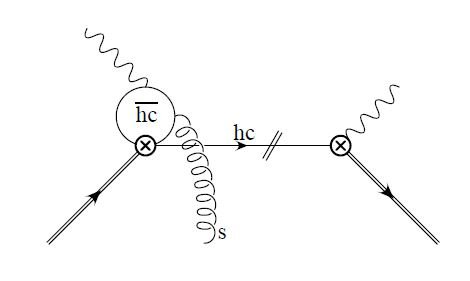
\includegraphics[width = 3in]{Q1Q7a.JPG}}
\subfloat[]{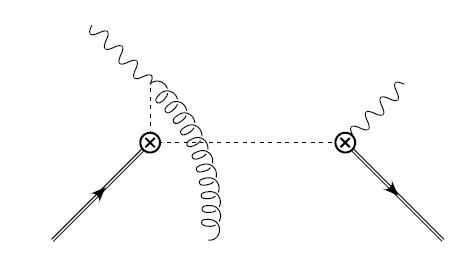
\includegraphics[width = 3in]{Q1Q7b.JPG}}\\
\caption{\label{fig:Q1Q7}Figure (a) represent the diagram arised by matching the $Q_1^q-Q_{7\gamma}$ operator to SCET. Figure (b) represents the diagram obtained by matching same process to HQET \cite{Benzke:2010js}.}
\end{figure}
The single resolved photon contribution of the operator $Q_{1}^q-Q_{7\gamma}$ is given by a non local soft function \cite{Benzke:2010js}
\begin{eqnarray}
\begin{aligned}\label{eqn:chapter3_single_resolved_photon_Q1Q7}
f_{17, q}(\omega, \mu)=\frac{2}{3} \int_{-\infty}^{\infty} \frac{d \omega_{1}}{\omega_{1}+i \varepsilon}\left[1-F\left(\frac{m_{q}^{2}-i \varepsilon}{\left(m_{b}+\omega\right) \omega_{1}}\right)\right] g_{17}\left(\omega, \omega_{1}, \mu\right),
\end{aligned}
\end{eqnarray}
where the penguin function $F$ is defined as 
\begin{eqnarray}\label{eqn:chapter3_penguin_fn}
F(x)=4 x \arctan ^{2}\left(\frac{1}{\sqrt{4 x-1}}\right).
\end{eqnarray}
The expansion of $F(x)$ around $x=0$ is
\begin{eqnarray}\label{eqn:chapter3_F_expansion}
1-F(x)=-\frac{1}{12 x}-\frac{1}{90 x^{2}}-\frac{1}{560 x^{3}}-\dots
\end{eqnarray}
The soft function $g_{17}\left(\omega, \omega_{1}, \mu\right)$  is defined as

\begin{align}\label{eqn:chapter3_suleadinhg_SSf}
g_{17}\left(\omega, \omega_{1}, \mu\right)=& \int \frac{d r}{2 \pi} e^{-i \omega_{1} r} \int \frac{d t}{2 \pi} e^{-i \omega t} \nonumber\\
& \times \frac{\left\langle\bar{B}\left|\left(\bar{h} S_{n}\right)(t n) \vec{\eta}\left(1+\gamma_{5}\right)\left(S_{n}^{\dagger} S_{\bar{n}}\right)(0) i \gamma_{\alpha}^{\perp} \bar{n}_{\beta}\left(S_{\bar{n}}^{\dagger} g G_{s}^{\alpha \beta} S_{\bar{n}}\right)(r \bar{n})\left(S_{\bar{n}}^{\dagger} h\right)(0)\right| \bar{B}\right\rangle}{2 M_{B}},\nonumber\\
\end{align}

where $r$ and $t$ are defined utilizing the topology of the HQET diagrams. For example, the weak vertex in the figure \ref{fig:Q1Q7} (b) is at $x=t n+x_{+}+x_{\perp}$ and the vertex of the soft gluon is defined at $y=r \bar{n}+y_{-}+y_{\perp}$. \par
The variables $\omega$ and $\omega_1$ in equation (\ref{eqn:chapter3_suleadinhg_SSf}) are defined using the light cone projections of parton momenta in $B$ meson. Since the total parton momenta including $b$ quark is equal to $M_B v$, the momentum of the partons in the $B$ meson can be given as 
\begin{eqnarray}
\sum_{i \neq b} n \cdot p_{i}+n \cdot k=\bar{\Lambda}, \quad \sum_{i \neq b} \bar{n} \cdot p_{i}+\bar{n} \cdot k=\bar{\Lambda},
\end{eqnarray}
where $k$ is the residual momentum and $\bar{\Lambda}= M_B-m_b$. Also, note that these light cone projections of parton momenta $n\cdot p_i$ and $\bar{n}\cdot p_i$ are non negative. This provides ($n.k$, $\bar{n}\cdot k)>-m_b$ for $i\neq b$. Besides, it implies $-\infty < n\cdot k\leq\bar{\Lambda}$ and $0 \leq n \cdot p_{i}<\infty$ in the heavy quark limit. These conditions are extended to $\bar{n}\cdot k$ and $\bar{n}\cdot p_i$ as well. Intuitively, the $\omega$ in soft function $g_{17}$ can be thought of as the residual momentum component $n\cdot k$ of the initial state heavy quark. The $\omega_1$ corresponds to either the momentum component $n\cdot p_g$ in final state $B$ meson or the component $-n\cdot p_g$ in initial state $B$ meson. Furthermore, this implies that $-\infty<\omega \leq \bar{\Lambda}$, and $-\infty<\omega_{1}<\infty$.
\par
The direct photon contributions and resolved photon contributions are combined into the final expression for $F_{17}$ in equation (\ref{eqn:chapter3_power_suppressed_terms}) as
\begin{eqnarray}\label{eqn:chapter3_F_17}
F_{17}\left(E_{\gamma}, \mu\right)=\frac{C_{F} \alpha_{s}(\mu)}{4 \pi}\left(-\frac{2}{3}\right) \int_{-p_{+}}^{\bar{\Lambda}} d \omega S(\omega, \mu)+\sum_{q=c, u} \delta_{q} \operatorname{Re} f_{17, q}\left(-p_{+}, \mu\right),
\end{eqnarray}\
where
\begin{eqnarray}
\delta_{q}=\frac{\operatorname{Re}\left[\lambda_{q} C_{1}(\mu)\left(-\lambda_{t}^{*}\right) C_{7 \gamma}^{*}(\mu)\right]}{\left|\lambda_{t}\right|^{2} \operatorname{Re}\left[C_{1}(\mu) C_{7 \gamma}^{*}(\mu)\right]}, \quad \lambda_{q}=V_{q b} V_{q s}^{*}.
\end{eqnarray}
\subsubsection{$Q_{7\gamma}-Q_{8g}$ contribution}
\vspace{-0.3cm}
The direct photon contribution from the operator pair $Q_{7\gamma}-Q_{8g}$ is given by
\begin{eqnarray}
F_{78}^{(a)}\left(E_{\gamma}, \mu\right)=\frac{C_{F} \alpha_{s}(\mu)}{4 \pi} \frac{m_{b}}{2 E_{\gamma}} \frac{10}{3} \int_{-p_{+}}^{\bar{\Lambda}} d \omega S(\omega, \mu)
\end{eqnarray}
The operator $Q_{8g}$ provides two SCET operators, and these operators are combined with the tree level SCET operator arising in $Q_{7\gamma}$. These two operators provide the $Q_{7\gamma}-Q_{8g}$ contribution.
Figure \ref{fig:Q1Q8} was obtained by matching the SCET operators onto HQET operators  \cite{Benzke:2010js}.
\begin{figure}[H]
\subfloat[]{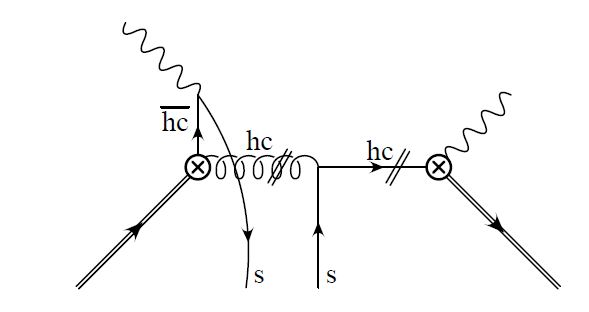
\includegraphics[width = 2.75in]{Q7Q8a.JPG}}
\subfloat[]{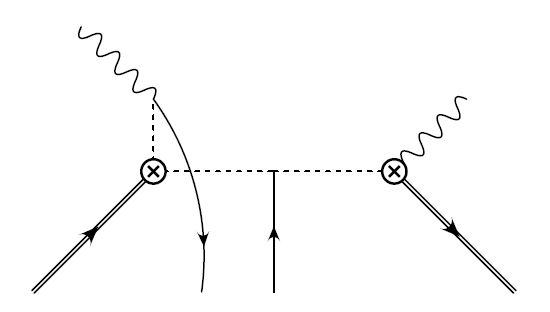
\includegraphics[width = 2.75in]{Q7Q8b.JPG}}\\
\subfloat[]{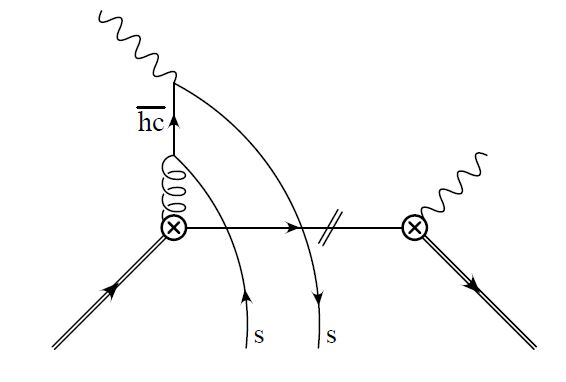
\includegraphics[width = 2.75in]{Q7Q8c.JPG}}
\subfloat[]{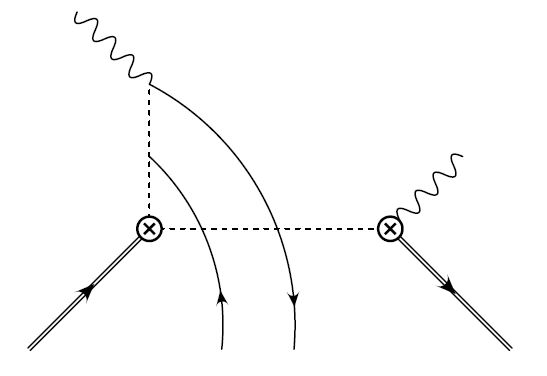
\includegraphics[width = 2.75in]{Q7Q8d.JPG}}
\caption{\label{fig:Q1Q8}Figure (a) and (c) represent the diagrams arised by matching the $Q_{7\gamma}-Q_{8g}$ operator to SCET. Figure (b) and (d) represents the diagrams obtained by matching same processes to HQET \cite{Benzke:2010js}.}
\end{figure} 
The contribution from the operator pair $Q_{7\gamma}-Q_{8g}$ to the photon spectrum is provided as \cite{Benzke:2010js}
\begin{eqnarray}
\begin{aligned}
F_{78}\left(E_{\gamma}, \mu\right)=& \frac{C_{F} \alpha_{s}(\mu)}{4 \pi} \frac{m_{b}}{2 E_{\gamma}} \frac{10}{3} \int_{-p_{+}}^{\bar{\Lambda}} d \omega S(\omega, \mu) \\
&+4 \pi \alpha_{s}(\mu) \frac{m_{b}}{2 E_{\gamma}} \operatorname{Re}\left[f_{78}^{(\mathrm{I})}\left(-p_{+}, \mu\right)+f_{78}^{(\mathrm{II})}\left(-p_{+}, \mu\right)\right],
\end{aligned}
\end{eqnarray}
where $f^{(\rm{I})}$ and $f^{(\rm{II})}$ are soft functions that encode the long distance physics. Unfortunately there is little information on these functions. The effect of these soft functions can be roughly approximated using \textit{vacuum insertion approximation} (VIA). In VIA, the matrix elements are evaluated by inserting vacuum states between light quark fields. Since the $Q_{7\gamma}-Q_{8g}$ operators involve light quark fields, the vacuum insertion model provides an estimate to the matrix element. Using the VIA model $f^{(\rm{I})}$ and $f^{(\rm{II})}$ as obtained as \cite{Benzke:2010js}

\begin{align}
\left.\int_{-\infty}^{\bar{\Lambda}} d \omega f_{78}^{(\mathrm{II})}(\omega, \mu)\right|_{\mathrm{VIA}} &=-e_{\mathrm{spec}} \frac{F^{2}(\mu)}{8}\left(1-\frac{1}{N_{c}^{2}}\right)\left\{\frac{1}{\lambda_{B}^{2}(\mu)}+2 \pi i \int_{0}^{\infty} d \omega \frac{\left[\phi_{+}^{B}(\omega, \mu)\right]^{2}}{\omega}\right\}\nonumber \\
\left.\int_{-\infty}^{\bar{\Lambda}} d \omega \operatorname{Re} f_{78}^{(\mathrm{II})}(\omega, \mu)\right|_{\mathrm{VIA}} &=-e_{\mathrm{spec}} \frac{F^{2}(\mu)}{8}\left(1-\frac{1}{N_{c}^{2}}\right) \frac{1}{\lambda_{B}^{2}(\mu)}, 
\end{align}

where $\lambda_{B}=\int_{0}^{\infty} d \omega \phi_{+}^{B}(\omega, \mu) / \omega$ and $\phi_{+}^{B}$ is the leading light cone distribution amplitude \cite{Grozin:1996pq}. The nonperturbative quantity $F(\mu)$ is the HQET matrix element that relates to the asymptotic value of $f_{B} \sqrt{M_{B}}|_{M_b\rightarrow \infty}$ and $f_B$ is the $B$ meson decay constant.
\vspace{-0.3cm}
\subsubsection{$Q_{8g}-Q_{8g}$ contribution} 
\vspace{-0.3cm}
The direct photon contribution of $Q_{8g}-Q_{8g}$ is given by \cite{Benzke:2010js}
\begin{eqnarray}\label{eqn:chapter3_Q8Q8_dir}
F_{88}^{(a)}\left(E_{\gamma}, \mu\right)=\frac{C_{F} \alpha_{s}(\mu)}{4 \pi}\left(\frac{m_{b}}{2 E_{\gamma}}\right)^{2} \int_{-p_{+}}^{\bar{\Lambda}} d \omega\left(\frac{2}{9} \ln \frac{m_{b}\left(\omega+p_{+}\right)}{\mu^{2}}+\frac{1}{9}-\frac{4}{9} c_{\mathrm{RS}}\right) S(\omega, \mu),
\end{eqnarray}
where $c_{\rm{RS}}$ is a scheme dependent coefficient. For instance, in $\bar{\rm{MS}}$ scheme $c_{\bar{\rm{MS}}}=0$. In the dimensional reduction scheme, which set $d=4$ instead of $d=4-2\epsilon$ for Dirac algebra, the $c_{\rm{DR}}=1$. The equation (\ref{eqn:chapter3_Q8Q8_dir}) is further simplified as 
\begin{eqnarray}
F_{88}^{(a)}\left(E_{\gamma}, \mu\right)=\frac{C_{F} \alpha_{s}(\mu)}{4 \pi}\left(\frac{m_{b}}{2 E_{\gamma}}\right)^{2} \int_{-p_{+}}^{\bar{\Lambda}} d \omega\left(\frac{2}{9} \ln \frac{m_{b}\left(\omega+p_{+}\right)}{\mu^{2}}-\frac{1}{3}\right) S(\omega, \mu),
\end{eqnarray}
The $Q_{8g}-Q_{8g}$ receives double resolved photon contributions. This is shown in the figure \ref{fig:Q8Q8}

\begin{figure}[H]
\subfloat[]{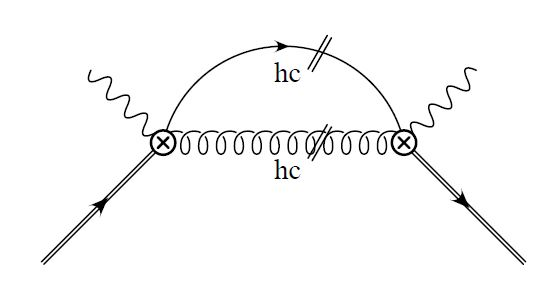
\includegraphics[width = 3in]{Q8Q8a.JPG}}
\subfloat[]{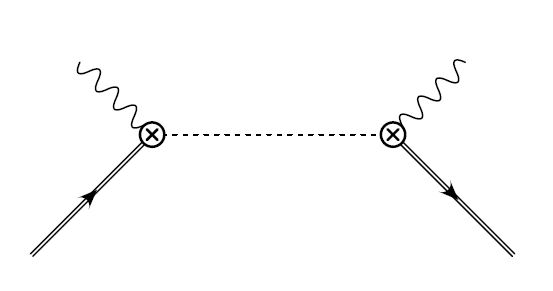
\includegraphics[width = 3in]{Q8Q8b.JPG}}\\
\subfloat[]{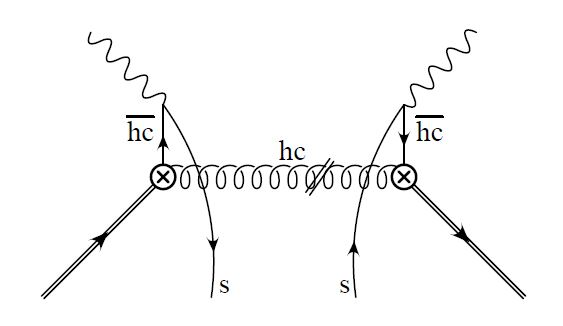
\includegraphics[width = 3in]{Q8Q8c.JPG}}
\subfloat[]{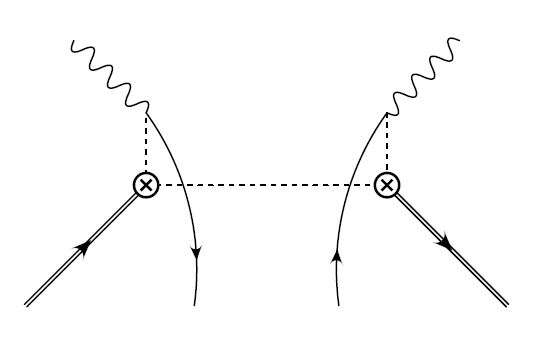
\includegraphics[width = 3in]{Q8Q8d.JPG}}
\caption{\label{fig:Q8Q8}Figure (a) and (c) represent the diagrams arised by matching the $Q_{8\gamma}-Q_{8g}$ operator to SCET. Figure (b) and (d) represents the diagrams obtained by matching same processes to HQET \cite{Benzke:2010js}.}
\end{figure} 
The double resolved contribution to the photon spectrum is given by \cite{Benzke:2010js}
\begin{eqnarray}
F_{88}^{(b)}\left(E_{\gamma}, \mu\right)=4 \pi \alpha_{s}(\mu)\left(\frac{m_{b}}{2 E_{\gamma}}\right)^{2} f_{88}\left(-p_{+}, \mu\right),
\end{eqnarray}
where $f_{88}$ encodes the long distance physics. This function is defined as 
\begin{eqnarray}
f_{88}(\omega, \mu)=\frac{2}{9} \int_{-\infty}^{\infty} \frac{d \omega_{1}}{\omega_{1}+i \varepsilon} \int_{-\infty}^{\infty} \frac{d \omega_{2}}{\omega_{2}-i \varepsilon} g_{88}^{\mathrm{cut}}\left(\omega, \omega_{1}, \omega_{2}, \mu\right),
\end{eqnarray}
where non-local matrix element $ g_{88}^{\mathrm{cut}}$ is given by

\begin{align}\label{eqn:chapter3_g88}
&g_{88}^{\mathrm{cut}}\left(\omega, \omega_{1}, \omega_{2}, \mu\right)\nonumber\\
=& \int \frac{d r}{2 \pi} e^{-i \omega_{1} r} \int \frac{d u}{2 \pi} e^{i \omega_{2} u} \int \frac{d t}{2 \pi} e^{-i \omega t}\nonumber \\
& \times \frac{\left\langle\bar{B}\left|\left(\bar{h} S_{n}\right)(t n) T^{A}\left(S_{n}^{\dagger} S_{\bar{n}}\right)(\operatorname{tn}) \bar{\Gamma}_{\bar{n}}\left(S_{\bar{n}}^{\dagger} s\right)(t n+u \bar{n})\left(\bar{s} S_{\bar{n}}\right)(r \bar{n}) \Gamma_{\bar{n}}\left(S_{\bar{n}}^{\dagger} S_{n}\right)(0) T^{A}\left(S_{n}^{\dagger} h\right)(0)\right| \bar{B}\right\rangle}{2 M_{B}}
\end{align}

The matrix element in equation (\ref{eqn:chapter3_g88}) is obtained by summing over soft intermediate states with strangeness $S=-1$ ($\mathcal{X}_{s}$).
\subsection{Resolved photon contributions to the total rate}
If the photon spectrum is integrated over a much larger interval in the phase space than the end point region (integrated rate), then the direct photon contributions can be further simplified. Typically, the direct photon contributions are given by a series of hard coefficients that are multiplyed by a set of forward $B$ meson matrix elements of local operators. The correction terms of order $\frac{\Lambda_{\rm{QCD}}}{m_b}$ are integrated to zero. This is due to the abscence of local gauge operators that can account such terms at the order $\frac{\Lambda_{\rm{QCD}}}{m_b}$. However, the resolved photon contributions do not reduced to such matrix elements of local operators \cite{Benzke:2010js}. The effects of these operators on total rate should be addressed by using non-local operators \cite{Lee:2006wn}\par
As shown in \cite{Benzke:2010js}, single resolved photon contributions arise from the operator pairs $Q_{8g}-Q_{7\gamma}$ and $Q_{1}^{c}-Q_{7\gamma}$. In addition, double resolved photon contributions arise from the operator pairs  $Q_{8g}-Q_{8g}$, $Q_{1}^{c}-Q_{1}^{c}$ and $Q_{1}^{c}-Q_{8g}$. Direct photon contributions arise from all the operator pairs.\par
The breakdown of the operators in leading order, next-to-leading order, and next-to-next-to-leading order in HQET power counting is as follows:
\begin{itemize}
  \item The contribution of the operators  $Q_{7\gamma}-Q_{7\gamma}$ is the leading power correction. 
  \item The operators $Q_{1}^{q}-Q_{7\gamma}$, $Q_{8g}-Q_{8g}$ and $Q_{8g}-Q_{7\gamma}$, are order $1/m_{b}$ in the power corrections. 
  \item The operators $Q_{1}^{c}-Q_{1}^{c}$ and $Q_{1}^{c}-Q_{8g}$ contribute at order $1/m^{2}_{b}$. Since our primary focus is on improving the order $1/m_b$ corrections, we do not consider these order $1/m^{2}_{b}$ operators in our analysis.
\end{itemize}
In the following, we discuss these order  $1/m_b$ corrections.
\subsection{Contribution from nonperturbative correction}\label{sec:nonpert_contr}
The function $\mathcal{F}_E$ quantifies the effects of resolved photon contributions to the total rate \cite{Benzke:2010js}
\begin{eqnarray}
\mathcal{F}_{E}(\Delta)=\frac{\Gamma(E_0)-\Gamma(E_0)|_{\rm{OPE}}}{\Gamma(E_0)|_{\rm{OPE}}},
\end{eqnarray} 
where $\Delta=m_{b}-2 E_{0}$. The $\Gamma(E_0)|_{\rm{OPE}}$ \cite{Misiak:2006zs} is obtained by a local operator product expansion, which does not consider the nonlocal power corrections from resolved photon contributions. The contribution from $1/m_b$ operators is
\begin{eqnarray}\label{eqn:chapter3_resolved_photon_err}
\begin{aligned}
\begin{aligned}
\mathcal{F}_{E}(\Delta)=& \frac{C_{1}(\mu)}{C_{7 \gamma}(\mu)} \frac{\Lambda_{17}\left(m_{c}^{2} / m_{b}, \mu\right)}{m_{b}}+\frac{C_{8 g}(\mu)}{C_{7 \gamma}(\mu)} 4 \pi \alpha_{s}(\mu) \frac{\Lambda_{78}^{\mathrm{spec}}(\mu)}{m_{b}} \\
&+\left(\frac{C_{8 g}(\mu)}{C_{7 \gamma}(\mu)}\right)^{2}\left[4 \pi \alpha_{s}(\mu) \frac{\Lambda_{88}(\Delta, \mu)}{m_{b}}-\frac{C_{F} \alpha_{s}(\mu)}{9 \pi} \ln \frac{\Delta}{m_{b}}\right]+\ldots,
\end{aligned}
\end{aligned}
\end{eqnarray}
where 

\begin{align}\label{eqn:chapter3_soft_functions}
\Lambda_{17}\left(\frac{m_{c}^{2}}{m_{b}}, \mu\right) &=e_{c} \operatorname{Re} \int_{-\infty}^{\infty} \frac{d \omega_{1}}{\omega_{1}}\left[1-F\left(\frac{m_{c}^{2}-i \varepsilon}{m_{b} \omega_{1}}\right)+\frac{m_{b} \omega_{1}}{12 m_{c}^{2}}\right] h_{17}\left(\omega_{1}, \mu\right)\nonumber \\
\Lambda_{78}^{\mathrm{spec}}(\mu) &=\operatorname{Re} \int_{-\infty}^{\infty} \frac{d \omega_{1}}{\omega_{1}+i \varepsilon} \int_{-\infty}^{\infty} \frac{d \omega_{2}}{\omega_{2}-i \varepsilon} h_{78}^{(5)}\left(\omega_{1}, \omega_{2}, \mu\right)\nonumber \\
\Lambda_{88}(\Delta, \mu) &=e_{s}^{2}\left[\int_{-\infty}^{\Lambda_{\mathrm{UV}}} \frac{d \omega_{1}}{\omega_{1}+i \varepsilon} \int_{-\infty}^{\Lambda_{\mathrm{UV}}} \frac{d \omega_{2}}{\omega_{2}-i \varepsilon} 2 h_{88}^{\mathrm{cut}}\left(\Delta, \omega_{1}, \omega_{2}, \mu\right)-\frac{C_{F}}{8 \pi^{2}} \Delta\left(\ln \frac{\Lambda_{\mathrm{UV}}}{\Delta}-1\right)\right].
\end{align}

The functions $h_{17}, h_{88}$ and $h_{78}$ are non-local HQET matrix elements that encode the long-distance nonperturbative effects\cite{Benzke:2010js}. These soft functions cannot be determined from the first principles, and the evaluation of their contribution to the total rate requires modeling. In the following, we provide a concise review regarding past evaluations their contribution. 
\vspace{-0.4cm}
\subsubsection{Estimating $\mathcal{F}_E|_{17}$}\label{sec:Q1Q7_cont}
\vspace{-0.2cm}
In equation (\ref{eqn:chapter3_soft_functions}) the soft function $h_{17}$ is defined as

\begin{eqnarray}\label{eqn:chapetr3_h_17}
\begin{aligned}
h_{17}\left(\omega_{1}, \mu\right) &=\int_{-\Delta}^{\bar{\Lambda}} d \omega g_{17}\left(\omega, \omega_{1}, \mu\right) \approx \int_{-\infty}^{\bar{\Lambda}} d \omega g_{17}\left(\omega, \omega_{1}, \mu\right) \\
&=\int \frac{d r}{2 \pi} e^{-i \omega_{1} r} \frac{\left\langle\bar{B}\left|\left(\bar{h} S_{\bar{n}}\right)(0) \slashed{\bar{n}} i \gamma_{\alpha}^{\perp} \bar{n}_{\beta}\left(S \frac{\dagger}{n} g G_{s}^{\alpha \beta} S_{\bar{n}}\right)(r \bar{n})\left(S_{\bar{n}}^{\dagger} h\right)(0)\right| \bar{B}\right\rangle}{2 M_{B}}
\end{aligned}
\end{eqnarray} 
\vspace{0.1cm}

The moments of the function $h_{17}$ in equation (\ref{eqn:chapetr3_h_17}) are related to the nonperturbative HQET parameters. Based on this feature, we can construct phenomenological models to describe this non-local function. For instance, in \cite{Benzke:2010js} there were several phenomenological models for function $h_{17}$ that are related to the zeroth moment of $h_{17}$ over $\omega_1$ ($\langle \omega_1^0 h_{17}(\omega_1)\rangle$). Consider the following model
\begin{eqnarray}\label{eqn:chapter3_old_model}
h_{17}\left(\omega_{1}, \mu\right)=\frac{2 \lambda_{2}}{\sqrt{2 \pi} \sigma} \frac{\omega_{1}^{2}-\Lambda^{2}}{\sigma^{2}-\Lambda^{2}} e^{-\frac{\omega_{1}^{2}}{2 \sigma^{2}}},
\end{eqnarray}
where $\sigma$ is the width of the Gaussian function and $\Lambda$ is a ad-hoc parameter. Scanning through different values for $\sigma$ and $\Lambda$ in $h_{17}$ the maximum and minimum values for $\Lambda_{17} $ obtained as \cite{Benzke:2010js}
\begin{eqnarray}
-60 \mathrm{MeV}<\Lambda_{17}<25 \mathrm{MeV}.
\end{eqnarray} 
Based on this estimate of $\Lambda_{17}$ the $\mathcal{F}_E|_{17}$ from equation (\ref{eqn:chapter3_resolved_photon_err})
\begin{eqnarray}
\mathcal{F}_E|_{17}=\frac{C_{1}(\mu)}{C_{7 \gamma}(\mu)} \frac{\Lambda_{17}\left(m_{c}^{2} / m_{b}, \mu\right)}{m_{b}}
\end{eqnarray}
\subsubsection{Estimating $\mathcal{F}_E|_{78}$}\label{subsec:F_78}
\vspace{-0.2cm}
The contribution of the operator pair $Q_{7\gamma}-Q_{8g}$ is obtained by using the flavor symmetry of the strong interaction. The flavor averaged estimate of the $\mathcal{F}_E|_{78}$ is given by \cite{Benzke:2010js}

\begin{eqnarray}\label{eqn:chapter3_78_contribution}
\left.\mathcal{F}_{E}^{\mathrm{avg}}(\Delta)\right|_{7 8}=-(1 \pm 0.3) \frac{\Delta_{0-}}{3},
\end{eqnarray}

where $\Delta_{0-}$ is the isospin asymmetry, which is given by

\begin{eqnarray}
\Delta_{0-}=\frac{\Gamma\left(\bar{B}^{0} \rightarrow X_{s} \gamma\right)-\Gamma\left(B^{-} \rightarrow X_{s} \gamma\right)}{\Gamma\left(\bar{B}^{0} \rightarrow X_{s} \gamma\right)+\Gamma\left(B^{-} \rightarrow X_{s} \gamma\right)}
\end{eqnarray}

Also, $\mathcal{F}_E|_{78}$ can be evaluated by using the vacuum insertion approximation (VIA). From equation (\ref{eqn:chapter3_resolved_photon_err})
 
\begin{eqnarray}
\mathcal{F}_E|_{78}= \frac{C_{8 g}(\mu)}{C_{7 \gamma}(\mu)} 4 \pi \alpha_{s}(\mu) \frac{\Lambda_{78}^{\mathrm{spec}}(\mu)}{m_{b}}, 
\end{eqnarray}

In the unbrocken $SU(3)$ flavor symmetry limit, the nonperturbative parameter $\Lambda_{78}^{\mathrm{spec}}$ is 
\begin{eqnarray}\label{eqn:chapter3_Lamda_78}
\left.\Lambda_{78}^{\mathrm{spec}}\right|_{S U(3)}=e_{\mathrm{spec}} \Lambda_{I=1}^{(8)},
\end{eqnarray}
where $e_{\rm{spec}}$ is the electric charge of the spectator quark (i.e $e_{\rm{spec}}=2/3$ for $B^{\pm}$ and $e_{\rm{spec}}=-1/3$ for $B^{0}(\bar{B}^{0})$). The soft function that encodes the long distance physics from $Q_{7\gamma}-Q_{8g}$ operator pair can be written as a $SU(3)$ octet matrix element. The Wigner-Ekchart theorem is used to decompose the matrix element  into isospin zero and isospin one components. The $\Lambda_{I=1}^{(8)}$ is the isospin 1 component of the $SU(3)$ octet. Using the VIA the estimate for $\Lambda_{I=1}^{(8)}$ is obtained as $\Lambda_{I=1}^{(8)}|_{\rm{VIA}}\in [-386,-35]\text{ MeV}$ \cite{Benzke:2010js}. This estimate is used in equation (\ref{eqn:chapter3_Lamda_78}) to obtain $\mathcal{F}_E|_{78}$.
\vspace{-0.3cm}
\subsubsection{Estimating $\mathcal{F}_E|_{88}$}\label{subsec:F_88}
\vspace{-0.2cm}
In equation (\ref{eqn:chapter3_resolved_photon_err}) the contribution from operator pair $Q_{8g}-Q_{8g}$ is 
\begin{eqnarray}\label{eqn:chapter3_Q8Q8}
\mathcal{F}_E|_{78}=\left(\frac{C_{8 g}(\mu)}{C_{7 \gamma}(\mu)}\right)^{2}\left[4 \pi \alpha_{s}(\mu) \frac{\Lambda_{88}(\Delta, \mu)}{m_{b}}-\frac{C_{F} \alpha_{s}(\mu)}{9 \pi} \ln \frac{\Delta}{m_{b}}\right].
\end{eqnarray}
\vspace{0.2cm}
Compared to the first term, the second term in the equation (\ref{eqn:chapter3_Q8Q8}) provides a very small contribution to the $\mathcal{F}_E|_{78}$ \cite{Benzke:2010js}. The first term in $\mathcal{F}_E|_{78}$ is defined using the nonperturabtive function $\Lambda_{88}$, which was defined in equation (\ref{eqn:chapter3_soft_functions}). Currently there is not much information on the soft function that describes $\Lambda_{88}$, and it is, however, estimated by \cite{Benzke:2010js} 
\begin{eqnarray}
\Lambda_{88}(\Delta, \mu) \approx e_{s}^{2} \Lambda(\mu), \quad \Lambda(\mu)>0,
\end{eqnarray}
where $\Lambda(\mu)$ is a parameter of order $\Lambda_{\mathrm{QCD}}$. The electromagnetic charge of the $s$ quark gives $e^2_s=\frac{1}{9}$. The range of the $\Lambda(\mu)$ is defined as $0<\Lambda(\mu)<1\text{ GeV}$ \cite{Benzke:2010js}. Based on this range the phenomenological estimate for the $\mathcal{F}_E|_{88}$ was obtained.
\vspace{-0.3cm}
\subsubsection{Phenomenological estimates of theoretical error}
\vspace{-0.2cm}
At order $1/m_{b}$, $\mathcal{F}_E$ depends on $Q_{1}-Q_{7\gamma}$, $Q_{8g}-Q_{8g}$ and $Q_{8g}-Q_{7\gamma}$; The contribution from each of these operators were obtained by Benzke \textit{et al.} (2010)\cite{Benzke:2010js}: 
\begin{eqnarray}\label{eqn:chapter3_error_est}
\begin{aligned}
&\left.\mathcal{F}_{E}\right|_{17} \in[-1.7,+4.0] \%\\
&\left.\mathcal{F}_{E}\right|_{88} \in[-0.3,+1.9] \%
\end{aligned}
\end{eqnarray}
and
\begin{eqnarray}
\begin{array}{l}
{\left.\mathcal{F}_{E}\right|_{78} ^{\mathrm{VIA}} \in[-2.8,-0.3] \%} \\
{\left.\mathcal{F}_{E}\right|_{78} ^{\mathrm{exp}} \in[-4.4,+5.6] \% \quad(95 \% \mathrm{CL})}
\end{array}
\end{eqnarray}
In total, the estimate for ${\cal F}_E$ is obtained by using both experimental and theoretical estimates of $\Lambda_{78}^{\rm{spec}}$. For instance, the 2010 theoretical estimate of uncertainty using VIA is \cite{Benzke:2010js}.

\begin{equation}\label{Fcurrentexp}
   -4.8 \%<\mathcal{F}_{E}(\Delta)<+5.6 \% \quad\left(\mathrm{VIA} \text { for } \Lambda_{78}^{\mathrm{spec}}\right).
\end{equation}
Here the estimate for $\mathcal{F}_E|^{\rm{VIA}}_{78}$ is obtained by plugging the value of $\Lambda_{I=1}^{(8)}|^{\rm{VIA}}$.\par
The 2010 estimate of $\Lambda_{78}^{\rm{spec}}$, which is obtained using isospin asymmetry $\Delta_{0-}$, is given by
\begin{eqnarray}\label{eqn:F78_using_exp}
-6.4 \%<\mathcal{F}_{E}(\Delta)<+11.5 \% \quad\left(\Lambda_{78}^{\mathrm{spec}} \text { from } \Delta_{0-}\right),
\end{eqnarray}
where $\Delta_{0-}=(-1.3 \pm 5.9) \%$, which was measured by BaBar collaboration \cite{Aubert:2005cua, Aubert:2007my}, and the uncertainty of $\Delta_{0-}$ is $95\%$ confidence level (CL) \cite{Benzke:2010js}. 

\section{The CP asymmetry}
The CP violation (CPV) due to direct photon in $\bar{B}\rightarrow X_s\gamma$ arises by the interference of a weak phases in the CKM matrix elements and the possible BSM corrections to Wilson coefficients with the strong phases arising in the process \cite{Kagan:1998bh}. These strong phases can be obtained by calculating the imaginary parts of the local operators in the effective Hamiltonian given in equation (\ref{eq:Weak Hamiltonian}). For instance, the imaginary parts first arise at $\mathcal{O}(\alpha_s)$ in loop diagrams that contains $c$ quarks or light partons \cite{Kagan:1998bh}.
The CP asymmetry is given by \cite{Benzke:2010tq},
\begin{equation}\label{data}
   {\cal A}_{X_s\gamma} 
   = \frac{\Gamma(\bar B\to X_s\gamma)-\Gamma(B\to X_{\bar s}\gamma)}%   
          {\Gamma(\bar B\to X_s\gamma)+\Gamma(B\to X_{\bar s}\gamma)} \,.
\end{equation}
In \cite{Benzke:2010tq} the SM estimate for CP asymmetry is provided as    
\begin{eqnarray}
-0.6\%< \mathcal{A}_{X_s\gamma}^{\rm{SM}}<2.8\%
\end{eqnarray}
This estimate is compared to the PDG average  of the experimental measurement $1.5 \% \pm 1.1 \%$ \cite{Tanabashi:2018oca}. These were first considered in \cite{Benzke:2010tq}.
The resolved photon contributions that arise in the photon spectrum is important to the analysis of the direct CP asymmetry.
\par
The experimental measurement of the CP asymmetry ($\mathcal{A}_{X_{s} \gamma}\left(E_{0}\right)$) depend on the photon cut $E_{\gamma}\geq E_0$. Where $E_0$ is in the range $1.9\text{ GeV}<E_0<2.2\text{ GeV}$, and $\Delta= m_b-2E_0= \rm{few}\times\Lambda_{\rm{QCD}}$ \cite{Benzke:2010tq}. This cut related CP asymmetry is known as \textit{partially inclusive} asymmetry \cite{Benzke:2010tq}. The direct photon contributions to the CP asymmetry can be expressed by using a power series in $\Delta/m_b$ and $\Lambda_{\rm{QCD}}/\Delta$. At the $\mathcal{O}(\alpha_s)$, the direct photon contribution to $\mathcal{A}_{X_{s} \gamma}$ is

\begin{eqnarray}\label{eqn:chapter3_dir_photon_CP}
   {\cal A}_{X_s\gamma}^{\rm dir}
   &=& \alpha_s\,\Bigg\{ \frac{40}{81}\,\mbox{Im}\frac{C_1}{C_{7\gamma}}
    - \frac49\,\mbox{Im}\frac{C_{8g}}{C_{7\gamma}}- \frac{40\Lambda_c}{9m_b}\,\mbox{Im}\bigg[(1+\epsilon_s)\,
    \frac{C_1}{C_{7\gamma}}\bigg] 
    + {\cal O}\bigg( \frac{\Lambda_{\rm QCD}^2}{m_b^2} \bigg) \Bigg\} \,, 
\end{eqnarray}
where the $C_1, C_{7\gamma}$ and $C_{8g}$ are the Wilson coefficients (effective couplings) of current-current four quark operator ($Q_{1}^q$), electromagnetic dipole operator ($Q_{7\gamma}$) and gluon dipole operator ($Q_{8g}$) respectively. Also, the parameter $\Lambda_{c}$ is defined as 
\begin{eqnarray}\label{eqn:chapter3_Lambda_C}
\Lambda_{c} \equiv \frac{m_{c}^{2}}{m_{b}}\left(1-\frac{2}{5} \ln \frac{m_{b}}{m_{c}}+\frac{4}{5} \ln ^{2} \frac{m_{b}}{m_{c}}-\frac{\pi^{2}}{15}\right),
\end{eqnarray}
The $\Lambda_c\sim\Lambda_{\rm{QCD}}$ is obtained by plugging $m_b=4.65\text{ GeV}$ and $m_c=1.13\text{ GeV}$ in equation (\ref{eqn:chapter3_Lambda_C}). Following from this we obtain $\Lambda_c\sim 0.38 \text{ GeV}$. The parameter $\epsilon_s$ is the ratio of CKM matrix elements, and it is defined as \cite{Kagan:1998bh}
\begin{eqnarray}
\epsilon_{s}=\frac{v_{u}}{v_{t}}=\frac{V_{u s}^{*} V_{u b}}{V_{t s}^{*} V_{t b}} \approx \lambda^{2}(i \eta-\rho)=O\left(10^{-2}\right),
\end{eqnarray}
where the parameters $\lambda,\rho$ and $\eta$ are Wolfenstein parameters defined as $\lambda=\sin \theta_{\mathrm{C}} \approx 0.22$ and $\rho, \eta=\mathcal{O}(1)$. Only the third term in the equation (\ref{eqn:chapter3_dir_photon_CP}) is non-zero in the SM. This term is triply suppressed by the $\alpha_s$, $\rm{Im}(\epsilon_s)$ and $(m_c/m_b)^2\sim \Lambda_{\rm{QCD}}/m_b$.

\subsection{Resolved photon contributions to the CP asymmetry}\label{sec:resolved_cp_A}
Using the factorization formula provided in equation (\ref{eqn:btoxgam_fact}) the effects of resolved photon operators to the partially inclusive CP asymmetry can be evaluated. For instance, these nonlocal effects arise from the interference of $Q_{7\gamma}-Q_{7\gamma}$ amplitude with $Q_{1}^{(u,c)}-Q_{7\gamma}$ and $Q_{7\gamma}-Q_{8g}$ amplitudes. Following from this, the resolved photon contribution to the CP asymmetry is obtained as
\begin{eqnarray}\label{eqn:chapter3_resolved_contr_CPA}
   {\cal A}_{X_s\gamma}^{\rm res}
   &=& \frac{\pi}{m_b}\,\bigg\{
    \mbox{Im}\bigg[(1+\epsilon_s)\,\frac{C_1}{C_{7\gamma}}\bigg]\,\tilde\Lambda_{17}^c 
    - \mbox{Im}\bigg[\epsilon_s\,\frac{C_1}{C_{7\gamma}}\bigg]\,\tilde\Lambda_{17}^u +\mbox{Im}\,\frac{C_{8g}}{C_{7\gamma}}\,
    4\pi\alpha_s\,\tilde\Lambda_{78}^{\bar B} \bigg\} \,,
\end{eqnarray}
where 
\begin{eqnarray}
\begin{aligned}
&\tilde{\Lambda}_{17}^{u}=\frac{2}{3} h_{17}(0)\\
&\tilde{\Lambda}_{17}^{c}=\frac{2}{3} \int_{4 m_{c}^{2} / m_{b}}^{\infty} \frac{d \omega}{\omega} f\left(\frac{m_{c}^{2}}{m_{b} \omega}\right) h_{17}(\omega)\\
&\tilde{\Lambda}_{78}^{\bar{B}}=2 \int_{-\infty}^{\infty} \frac{d \omega}{\omega}\left[h_{78}^{(1)}(\omega, \omega)-h_{78}^{(1)}(\omega, 0)\right]
\end{aligned}
\end{eqnarray}
and 
\begin{eqnarray}
f(x)=2 x \ln \frac{1+\sqrt{1-4 x}}{1-\sqrt{1-4 x}}.
\end{eqnarray}

In the unbroken $SU(3)$ limit, the $\tilde{\Lambda}_{78}$ is defined as
\begin{eqnarray}
\tilde{\Lambda}_{78}^{\bar{B}} \approx e_{\text {spec }} \tilde{\Lambda}_{78} \approx e_{\text {spec }} \frac{2 f_{B}^{2} M_{B}}{9} \int_{0}^{\infty} d \omega \frac{\left[\phi_{+}^{B}(\omega)\right]^{2}}{\omega},
\end{eqnarray}
where the $f_{B}$ is the $B$ meson decay constant and it is evaluated as $f_{B}\approx 193\text{ MeV}$ \cite{Benzke:2010tq}. The $\phi_{+}^{B}$ is the leading light cone distribution amplitude \cite{Grozin:1996pq}. Using the models provided in sections \ref{sec:Q1Q7_cont} and \ref{subsec:F_88} the parameters $\tilde{\Lambda}_{ij}$ can be obtained \cite{Benzke:2010tq}
\vspace*{-0.6cm}
\begin{eqnarray}
\begin{aligned}
-330 \mathrm{MeV} &<\tilde{\Lambda}_{17}^{u}<+525 \mathrm{MeV}, \\
-9 \mathrm{MeV} &<\tilde{\Lambda}_{17}^{c}<+11 \mathrm{MeV}, \\
17 \mathrm{MeV} &<\tilde{\Lambda}_{78}<190 \mathrm{MeV}.
\end{aligned}
\vspace*{-0.5cm}
\end{eqnarray}
The complete theoretical estimate of the CP asymmetry is obtained by  combining the direct and the resolved photon contributions. Therefore, the SM estimate of the CP asymmetry is obtained by using the expressions in equations (\ref{eqn:chapter3_dir_photon_CP}) and (\ref{eqn:chapter3_resolved_contr_CPA}), and they provide
\vspace*{-0.6cm}
\begin{eqnarray}\label{eqn:resolved_p_cont_CP}
\begin{aligned}
\mathcal{A}_{X_{s} \gamma}^{\mathrm{SM}} & \approx \pi\left|\frac{C_{1}}{C_{7 \gamma}}\right| \operatorname{Im} \epsilon_{s}\left(\frac{\tilde{\Lambda}_{17}^{u}-\tilde{\Lambda}_{17}^{c}}{m_{b}}+\frac{40 \alpha_{s}}{9 \pi} \frac{\Lambda_{c}}{m_{b}}\right) \\
&=\left(1.15 \times \frac{\tilde{\Lambda}_{17}^{u}-\tilde{\Lambda}_{17}^{c}}{300 \mathrm{MeV}}+0.71\right) \%,
\end{aligned}
\end{eqnarray}

where the following estimates for the Wolfenstein parameters are used: $\lambda=0.2254$, $\rho=0.144$, $\eta=0.342$. The Wilson coefficients are evaluated at $\mu=2\text{ GeV}$, they are provided as: $C_{1}=1.204$, $C_{7\gamma}=-0.381$ and $C_{8g}=-0.175$ \cite{Benzke:2010tq}. 
\section{Reevaluating the resolved photon contributions}\label{sec:reeval_resolved_photon_cont}

\subsection{Updates on the $\mathcal{F}_{E}|_{78}$}
A recent update on $\Delta_{0-}$ from Belle \cite{Watanuki:2018xxg} provide $\Delta_{0-}=[-0.48\pm 1.49(\rm{stat})\pm 0.97(\rm{sys})\pm1.15(f_{+-}/f_{00})]\%$, where the last uncertainty is coming from the uncertainties attached to the production ratio of $B^+B^-$ to $B^0\bar{B}^0$ in $\Upsilon(4S)$ decays \cite{Gunawardana:2019gep}. The PDG average is $\Delta_{0-}=(-0.6\pm 2.0)\%$ \cite{Aubert:2005cua, Watanuki:2018xxg, Aubert:2007my}. As shown in the equation (\ref{eqn:F78_using_exp}), the uncertainty of the $\Delta_{0-}$ is calculated in $95\%$ CL. Using this in equation (\ref{eqn:chapter3_78_contribution}) we find
\vspace*{-0.6cm}
\begin{eqnarray}\label{eqn:chapter3_78_update}
\mathcal{F}_{E}|_{78} ^{\mathrm{exp}}\in [-1.4,+2] \%.
\vspace*{-0.5cm}
\end{eqnarray}

Comparing the estimates found in equation (\ref{eqn:chapter3_error_est}) and (\ref{eqn:chapter3_78_update}), we find that the currently the largest contribution to the ${\cal F} _E$ comes from the operator pair $Q_{1}^{q}-Q_{7\gamma}$. Therefore, reducing the theoretical error generated by this operator pair is essential for the precise calculation of the branching ratio.